% Apresentações em widescreen. Outros valores possíveis: 1610, 149, 54, 43 e 32.
% Por padrão, as apresentações são no formato 4:3 (sem o aspectratio).
\documentclass[aspectratio=43]{beamer}

\usetheme{Antibes}
\usecolortheme{default}
\usefonttheme[onlymath]{serif}			% para fontes matemáticas
% Enconte mais temas e cores em http://www.hartwork.org/beamer-theme-matrix/
% Veja também http://deic.uab.es/~iblanes/beamer_gallery/index.html
\bibliography{references}
% Customizações de Cores: fg significa cor do texto e bg é cor do fundo
\setbeamercolor{normal text}{fg=black}
\setbeamercolor{alerted text}{fg=red}
\setbeamercolor{author}{fg=black}
\setbeamercolor{institute}{fg=blue}
\setbeamercolor{date}{fg=black}
\setbeamercolor{frametitle}{fg=white}
\setbeamercolor{framesubtitle}{fg=brown}
\setbeamercolor{block title}{bg=blue, fg=white}		%Cor do título
\setbeamercolor{block body}{bg=gray, fg=darkgray}	%Cor do texto(bg= fundo; fg=texto)

% ---
% PACOTES
% ---
\usepackage[alf]{abntex2cite}		% Citações padrão ABNT
\usepackage[brazil]{babel}		% Idioma do documento
\usepackage{color}			% Controle das cores
\usepackage[T1]{fontenc}		% Selecao de codigos de fonte.
\usepackage{graphicx}			% Inclusão de gráficos
\usepackage[utf8]{inputenc}		% Codificacao do documento (conversão automática dos acentos)
\usepackage{gensymb}
\usepackage{txfonts}			% Fontes virtuais
% ---

% --- Informações do documento ---
\title{Relatório sobre o OrchFlow}
\author{
	Angelo Silva
	\and Dante Mesquita Neto
	\and Jônatas Bonventti
	\and Pedro
}
\institute{Instituto Federal de Educação, Ciência e Tecnologia de São Paulo Câmpus Boituva
	    \par
	    Curso de Análise e Desenvolvimento de sistemas}
\date{\today, v-1.0.0}
% ---

% -----------------INÍCIO DO DOCUMENTO --------------------------------------
\begin{document}

\frame{\titlepage}

\begin{frame}{Introdução}
\section{Introdução}

Devido a tomadas de decisão imaturas, partes do software acabaram ao longo da primeira implantação do sistema levando um rumo não focado em qualidade, mas sim em simplesmente finalizar a implantação.
Através de técnicas simples de desenvolvimento de software e devops, tentamos reescrever pequenos trechos da aplicação, refatorando o sistema.
\end{frame}

\begin{frame}{Docker e contêineres}
\section{Docker e contêineres}
\begin{figure}[H]
    \label{figure_arquitetura_container}
    \centering
    \caption{Arquitetura dos contêineres}
    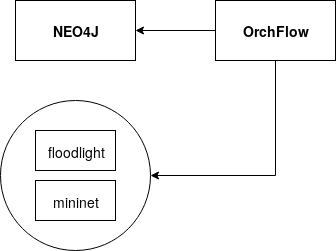
\includegraphics[scale=0.6]{arquitetura_container.png}
    \hfill
\end{figure}
\end{frame}

\begin{frame}{Receptibilidade de desenvolvedores}
\section{Receptibilidade de desenvolvedores}
Implementando uma infraestrutura baseada em contêineres conseguimos reduzir consideravelmente a receptibilidade de novos programadores no projeto, como cada serviço fica contido dentro do seu próprio contêiner, configurar um ambiente de desenvolvimento se torna algo até mesmo monótono, não se perde mais tempo tentando entender configurações mágicas que, uma vez não documentadas, são esquecidas.
\end{frame}

\begin{frame}{Acoplamento de configurações}
\section{Acoplamento de configurações}
Um outro problema que foi notado ao iniciar o projeto de manutenção do OrchFlow, que, somado a uma arquitetura baseada em contêineres poderia tornar o desenvolvimento mais rápido, é o acoplamento de configurações, existem chaves de API e configurações de banco de dados direto no código da aplicação, isso torna a arquitetura OrchFlow um impedimento para novos programadores.\\
Para solucionar o problema, criamos um pacote de configuração, centralizando todas as configurações do sistema.
\end{frame}

\begin{frame}{Padrões de nomeação}
\section{Padrões de nomeação}
Foi trabalhada durante a manutenção do sistema um novo padrão de nomeação, problemas com nomeação de classes e camadas foram solucionados, unificando o idioma para o inglês americano.
\end{frame}

\begin{frame}{Problemas com separação de camadas}
\section{Problemas com separação de camadas}
\begin{figure}[H]
    \label{figure_arquitetura_camadas}
    \centering
    \caption{Arquitetura de camadas}
    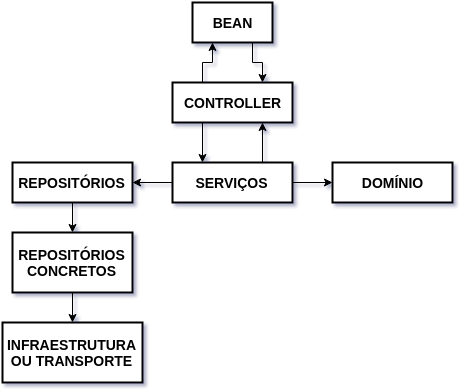
\includegraphics[scale=0.4]{arquitetura_camadas.png}
    \hfill
\end{figure}
\end{frame}

% --- O comando \allowframebreaks ---
% Se o conteúdo não se encaixa em um quadro, a opção allowframebreaks instrui
% beamer para quebrá-lo automaticamente entre dois ou mais quadros,
% mantendo o frametitle do primeiro quadro (dado como argumento) e acrescentando
% um número romano ou algo parecido na continuação.no
% \begin{frame}[allowframebreaks]{Referências}
% \end{frame}

% ----------------- FIM DO DOCUMENTO -----------------------------------------
\end{document}
